%%%%%%%%%%%%%%%%%%%%%%%%%%%%%%%%%%%%%%%%%%%%%%%%%%%%%%%%%%%%%%%
%
% Welcome to writeLaTeX --- just edit your LaTeX on the left,
% and we'll compile it for you on the right. If you give
% someone the link to this page, they can edit at the same
% time. See the help menu above for more info. Enjoy!
%
%%%%%%%%%%%%%%%%%%%%%%%%%%%%%%%%%%%%%%%%%%%%%%%%%%%%%%%%%%%%%%%

% --------------------------------------------------------------
% This is all preamble stuff that you don't have to worry about.
% Head down to where it says "Start here"
% --------------------------------------------------------------
 
\documentclass[12pt]{article}
 
\usepackage[margin=1in]{geometry}
\usepackage{amsmath,amsthm,amssymb}

\usepackage{listings}
\usepackage{xcolor}

\usepackage{cancel}
\usepackage{caption}
\usepackage{subcaption}
\usepackage{enumitem}

\usepackage{tikz}
\usetikzlibrary{shapes,positioning}

\tikzset{ell/.style={circle,draw,minimum height=0.5cm,minimum width=0.5cm,inner sep=0.2cm}}

%New colors defined below
\definecolor{codegreen}{rgb}{0,0.6,0}
\definecolor{codegray}{rgb}{0.5,0.5,0.5}
\definecolor{codepurple}{rgb}{0.58,0,0.82}
\definecolor{backcolour}{rgb}{0.95,0.95,0.92}

%Code listing style named "mystyle"
\lstdefinestyle{mystyle}{
  backgroundcolor=\color{backcolour}, commentstyle=\color{codegreen},
  keywordstyle=\color{magenta},
  numberstyle=\tiny\color{codegray},
  stringstyle=\color{codepurple},
  basicstyle=\ttfamily\footnotesize,
  breakatwhitespace=false,         
  breaklines=true,                 
  captionpos=b,                    
  keepspaces=true,                 
  numbers=left,                    
  numbersep=5pt,                  
  showspaces=false,                
  showstringspaces=false,
  showtabs=false,                  
  tabsize=2
}

%"mystyle" code listing set
\lstset{style=mystyle}

 
\newcommand{\N}{\mathbb{N}}
\newcommand{\Z}{\mathbb{Z}}
 
\newenvironment{theorem}[2][Theorem]{\begin{trivlist}
\item[\hskip \labelsep {\bfseries #1}\hskip \labelsep {\bfseries #2.}]}{\end{trivlist}}
\newenvironment{lemma}[2][Lemma]{\begin{trivlist}
\item[\hskip \labelsep {\bfseries #1}\hskip \labelsep {\bfseries #2.}]}{\end{trivlist}}
\newenvironment{exercise}[2][Exercise]{\begin{trivlist}
\item[\hskip \labelsep {\bfseries #1}\hskip \labelsep {\bfseries #2.}]}{\end{trivlist}}
\newenvironment{problem}[2][Problem]{\begin{trivlist}
\item[\hskip \labelsep {\bfseries #1}\hskip \labelsep {\bfseries #2.}]}{\end{trivlist}}
\newenvironment{question}[2][Question]{\begin{trivlist}
\item[\hskip \labelsep {\bfseries #1}\hskip \labelsep {\bfseries #2.}]}{\end{trivlist}}
\newenvironment{corollary}[2][Corollary]{\begin{trivlist}
\item[\hskip \labelsep {\bfseries #1}\hskip \labelsep {\bfseries #2.}]}{\end{trivlist}}

\newenvironment{solution}{\begin{proof}[Solution]}{\end{proof}}
 
\begin{document}
 
% --------------------------------------------------------------
%                         Start here
% --------------------------------------------------------------
 
\title{Homework 4}%replace X with the appropriate number
\author{Mengxiang Jiang\\ %replace with your name
CSEN 5336 Analysis of Algorithms} %if necessary, replace with your course title
 
\maketitle
 
\begin{problem}{1} %You can use theorem, exercise, problem, or question here.  Modify x.yz to be whatever number you are proving
    Find the prefix function $\pi$ for the pattern $P$ = ``tortoise" for the Knuth-Morris-Pratt Algorithm. Find
    out the status $q$ at different steps while searching the pattern in the text $T$ = ``distortion tortoise
    tortilla".\\\\
Prefix function $\pi[1\ldots m]$:\\\\
\begin{tabular}[b]{|c|c|c|c|c|c|c|c|c|} 
  \hline
  $i$ & 1 & 2 & 3 & 4 & 5 & 6 & 7 & 8 \\
  \hline
  $p[i]$ & t & o & r & t & o & i & s & e\\
  \hline
  $\pi[i]$ & 0 & 0 & 0 & 1 & 2 & 0 & 0 & 0\\
  \hline
\end{tabular}
\\Current state values:
\begin{table}[ht!]
From $i=1\ldots 19$:\\
\begin{tabular}[b]{|c|c|c|c|c|c|c|c|c|c|c|c|c|c|c|c|c|c|c|c|}
  \hline
  $i$ & 1 & 2 & 3 & 4 & 5 & 6 & 7 & 8 & 9 
    & 10 & 11 & 12 & 13 & 14 & 15 & 16 & 17 & 18 & 19\\
    \hline
  $T[i]$ & d & i & s & t & o & r & t & i & o 
        & n &   & t & o & r & t & o & i & s & e \\
  \hline
  $q[i]$ & 0 & 0 & 0 & 1 & 2 & 3 & 4 & \cancel{1} 0 & 0
        & 0 & 0 & 1 & 2 & 3 & 4 & 5 & 6 & 7 & \cancel{8} 0 \\
  \hline
\end{tabular}
\\From $i=20\ldots 28$:\\
\begin{tabular}[b]{|c|c|c|c|c|c|c|c|c|c|}
    \hline
    $i$ & 20 & 21 & 22 & 23 & 24 & 25 & 26 & 27 & 28 \\
    \hline
    $T[i]$ &   & t & o & r & t & i & l & l & a\\
    \hline
    $q[i]$ & 0 & 1 & 2 & 3 & 4 & \cancel{1} 0 & 0 & 0 & 0\\
    \hline
  \end{tabular}
\end{table}
\\one valid shift at $i = 19$ $\rightarrow$ shift of $i - m = 19 - 8 = 11$.
\end{problem}
\pagebreak
\begin{problem}{2}
Find the maximum flow in the flow network shown in figure 1. In the flow network $s$ is the
source vertex and $t$ is the destination vertex. The capacity of each of the edges are given in the
figure.
\begin{figure}[ht!]
    \caption{Flow Network}
    \centering
    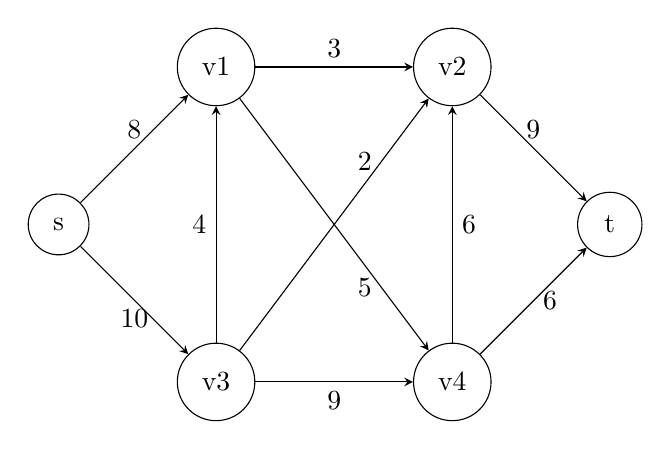
\begin{tikzpicture}[>=stealth]
        \node[ell] (s) at (0,0) {s};
        \node[ell] (v1) at (2,2) {v1};
        \node[ell] (v2) at (5,2) {v2};
        \node[ell] (v3) at (2,-2) {v3};
        \node[ell] (v4) at (5,-2) {v4};
        \node[ell] (t) at (7,0) {t};

        \draw [->] (s) to []node[above]{8} (v1);
        \draw [->] (s) to []node[below]{10} (v3);
        \draw [->] (v1) to []node[above]{3} (v2);
        \draw [->] (v1) to []node[left, near end]{5} (v4);
        \draw [->] (v2) to []node[above]{9} (t);
        \draw [->] (v3) to []node[left]{4} (v1);
        \draw [->] (v3) to []node[left, near end]{2} (v2);
        \draw [->] (v3) to []node[below]{9} (v4);
        \draw [->] (v4) to []node[right]{6} (v2);
        \draw [->] (v4) to []node[right]{6} (t);
    \end{tikzpicture}
\end{figure}

\begin{figure}[ht!]
    \captionsetup{labelformat=empty}
    \caption{Augmenting path with $f'=6$}
    \centering
    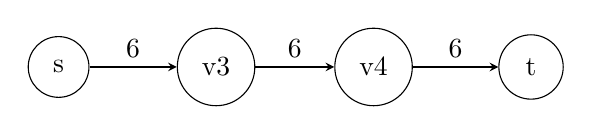
\begin{tikzpicture}[>=stealth]
        \node[ell] (s) at (0,0) {s};
        \node[ell] (v3) at (2,0) {v3};
        \node[ell] (v4) at (4,0) {v4};
        \node[ell] (t) at (6,0) {t};

        \draw [->] (s) to []node[above]{6} (v3);
        \draw [->] (v3) to []node[above]{6} (v4);
        \draw [->] (v4) to []node[above]{6} (t);
    \end{tikzpicture}
\end{figure}

\begin{figure}[ht!]
    \begin{subfigure}{0.5\textwidth}
    \captionsetup{labelformat=empty}
    \caption{$G_{f}$}
    \centering
    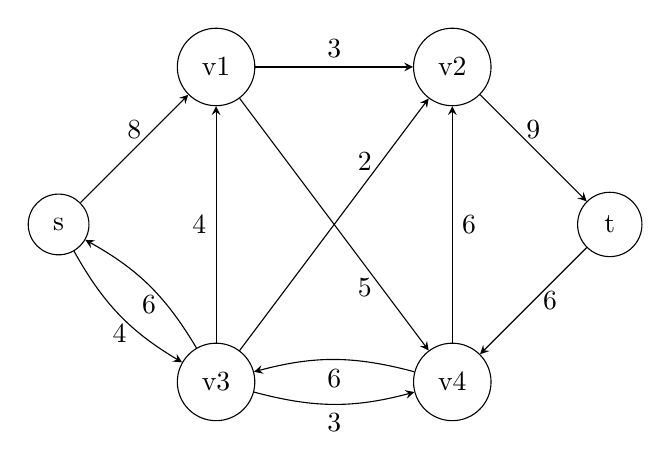
\begin{tikzpicture}[>=stealth]
        \node[ell] (s) at (0,0) {s};
        \node[ell] (v1) at (2,2) {v1};
        \node[ell] (v2) at (5,2) {v2};
        \node[ell] (v3) at (2,-2) {v3};
        \node[ell] (v4) at (5,-2) {v4};
        \node[ell] (t) at (7,0) {t};

        \draw [->] (s) to []node[above]{8} (v1);
        \draw [->] (s) to [bend right=15]node[below]{4} (v3);
        \draw [->] (v3) to [bend right=15]node[below]{6} (s);
        \draw [->] (v1) to []node[above]{3} (v2);
        \draw [->] (v1) to []node[left, near end]{5} (v4);
        \draw [->] (v2) to []node[above]{9} (t);
        \draw [->] (v3) to []node[left]{4} (v1);
        \draw [->] (v3) to []node[left, near end]{2} (v2);
        \draw [->] (v3) to [bend right=15]node[below]{3} (v4);
        \draw [->] (v4) to [bend right=15]node[below]{6} (v3);
        \draw [->] (v4) to []node[right]{6} (v2);
        \draw [->] (t) to []node[right]{6} (v4);
    \end{tikzpicture}
    \end{subfigure}
    \begin{subfigure}{0.5\textwidth}
    \captionsetup{labelformat=empty}
    \caption{Augmenting path with $f'=3$}
    \centering
    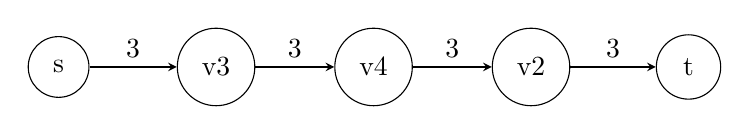
\begin{tikzpicture}[>=stealth]
        \node[ell] (s) at (0,0) {s};
        \node[ell] (v3) at (2,0) {v3};
        \node[ell] (v4) at (4,0) {v4};
        \node[ell] (v2) at (6,0) {v2};
        \node[ell] (t) at (8,0) {t};

        \draw [->] (s) to []node[above]{3} (v3);
        \draw [->] (v3) to []node[above]{3} (v4);
        \draw [->] (v4) to []node[above]{3} (v2);
        \draw [->] (v2) to []node[above]{3} (t);
    \end{tikzpicture}
    \end{subfigure}
\end{figure}

\begin{figure}[ht!]
    \begin{subfigure}{0.5\textwidth}
    \captionsetup{labelformat=empty}
    \caption{$G_{f1}$}
    \centering
    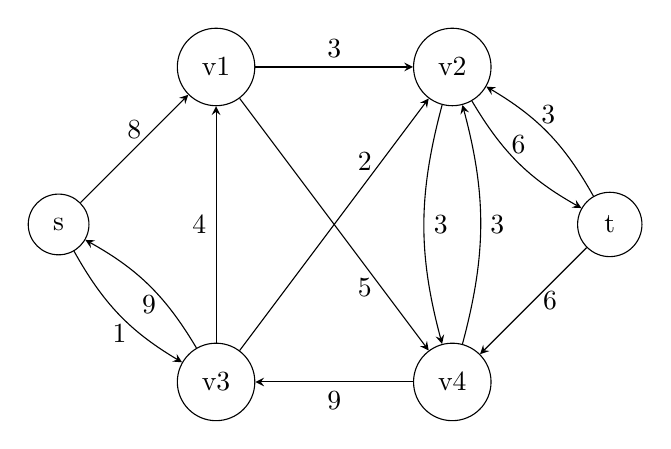
\begin{tikzpicture}[>=stealth]
        \node[ell] (s) at (0,0) {s};
        \node[ell] (v1) at (2,2) {v1};
        \node[ell] (v2) at (5,2) {v2};
        \node[ell] (v3) at (2,-2) {v3};
        \node[ell] (v4) at (5,-2) {v4};
        \node[ell] (t) at (7,0) {t};

        \draw [->] (s) to []node[above]{8} (v1);
        \draw [->] (s) to [bend right=15]node[below]{1} (v3);
        \draw [->] (v3) to [bend right=15]node[below]{9} (s);
        \draw [->] (v1) to []node[above]{3} (v2);
        \draw [->] (v1) to []node[left, near end]{5} (v4);
        \draw [->] (v2) to [bend right=15]node[above]{6} (t);
        \draw [->] (t) to [bend right=15]node[above]{3} (v2);
        \draw [->] (v3) to []node[left]{4} (v1);
        \draw [->] (v3) to []node[left, near end]{2} (v2);
        \draw [->] (v4) to []node[below]{9} (v3);
        \draw [->] (v4) to [bend right=15]node[right]{3} (v2);
        \draw [->] (v2) to [bend right=15]node[right]{3} (v4);
        \draw [->] (t) to []node[right]{6} (v4);
    \end{tikzpicture}
    \end{subfigure}
    \begin{subfigure}{0.5\textwidth}
    \captionsetup{labelformat=empty}
    \caption{Augmenting path with $f'=3$}
    \centering
    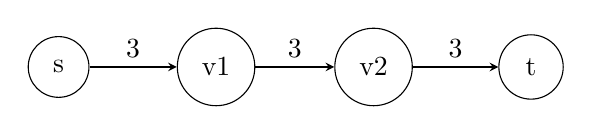
\begin{tikzpicture}[>=stealth]
        \node[ell] (s) at (0,0) {s};
        \node[ell] (v1) at (2,0) {v1};
        \node[ell] (v2) at (4,0) {v2};
        \node[ell] (t) at (6,0) {t};

        \draw [->] (s) to []node[above]{3} (v1);
        \draw [->] (v1) to []node[above]{3} (v2);
        \draw [->] (v2) to []node[above]{3} (t);
    \end{tikzpicture}
    \end{subfigure}
\end{figure}

\begin{figure}[ht!]
    \begin{subfigure}{0.5\textwidth}
    \captionsetup{labelformat=empty}
    \caption{$G_{f2}$}
    \centering
    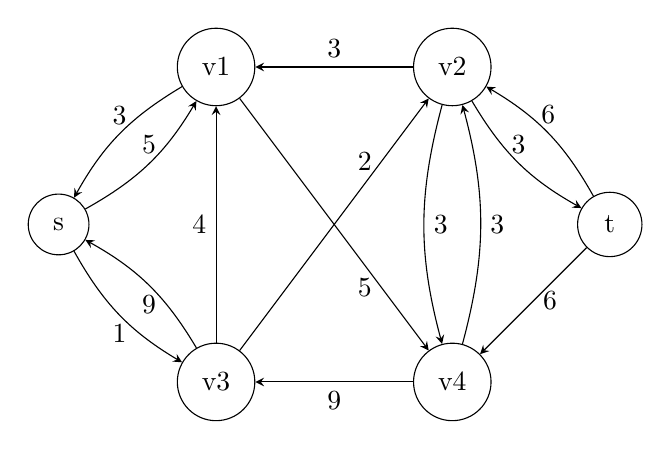
\begin{tikzpicture}[>=stealth]
        \node[ell] (s) at (0,0) {s};
        \node[ell] (v1) at (2,2) {v1};
        \node[ell] (v2) at (5,2) {v2};
        \node[ell] (v3) at (2,-2) {v3};
        \node[ell] (v4) at (5,-2) {v4};
        \node[ell] (t) at (7,0) {t};

        \draw [->] (s) to [bend right=15]node[above]{5} (v1);
        \draw [->] (v1) to [bend right=15]node[above]{3} (s);
        \draw [->] (s) to [bend right=15]node[below]{1} (v3);
        \draw [->] (v3) to [bend right=15]node[below]{9} (s);
        \draw [->] (v2) to []node[above]{3} (v1);
        \draw [->] (v1) to []node[left, near end]{5} (v4);
        \draw [->] (v2) to [bend right=15]node[above]{3} (t);
        \draw [->] (t) to [bend right=15]node[above]{6} (v2);
        \draw [->] (v3) to []node[left]{4} (v1);
        \draw [->] (v3) to []node[left, near end]{2} (v2);
        \draw [->] (v4) to []node[below]{9} (v3);
        \draw [->] (v4) to [bend right=15]node[right]{3} (v2);
        \draw [->] (v2) to [bend right=15]node[right]{3} (v4);
        \draw [->] (t) to []node[right]{6} (v4);
    \end{tikzpicture}
    \end{subfigure}
    \begin{subfigure}{0.5\textwidth}
    \captionsetup{labelformat=empty}
    \caption{Augmenting path with $f'=3$}
    \centering
    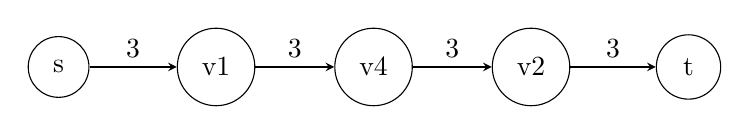
\begin{tikzpicture}[>=stealth]
        \node[ell] (s) at (0,0) {s};
        \node[ell] (v1) at (2,0) {v1};
        \node[ell] (v4) at (4,0) {v4};
        \node[ell] (v2) at (6,0) {v2};
        \node[ell] (t) at (8,0) {t};

        \draw [->] (s) to []node[above]{3} (v1);
        \draw [->] (v1) to []node[above]{3} (v4);
        \draw [->] (v4) to []node[above]{3} (v2);
        \draw [->] (v2) to []node[above]{3} (t);
    \end{tikzpicture}
    \end{subfigure}
\end{figure}

\begin{figure}[ht!]
    \begin{subfigure}{0.5\textwidth}
    \captionsetup{labelformat=empty}
    \caption{$G_{f3}$}
    \centering
    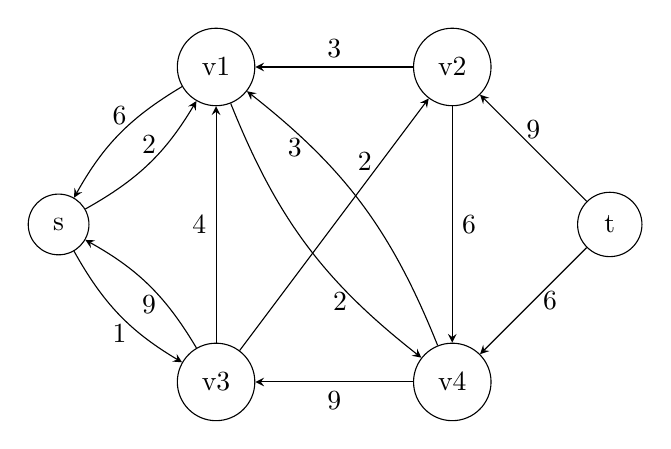
\begin{tikzpicture}[>=stealth]
        \node[ell] (s) at (0,0) {s};
        \node[ell] (v1) at (2,2) {v1};
        \node[ell] (v2) at (5,2) {v2};
        \node[ell] (v3) at (2,-2) {v3};
        \node[ell] (v4) at (5,-2) {v4};
        \node[ell] (t) at (7,0) {t};

        \draw [->] (s) to [bend right=15]node[above]{2} (v1);
        \draw [->] (v1) to [bend right=15]node[above]{6} (s);
        \draw [->] (s) to [bend right=15]node[below]{1} (v3);
        \draw [->] (v3) to [bend right=15]node[below]{9} (s);
        \draw [->] (v2) to []node[above]{3} (v1);
        \draw [->] (v1) to [bend right=15]node[left, near end]{2} (v4);
        \draw [->] (v4) to [bend right=15]node[left, near end]{3} (v1);
        \draw [->] (t) to []node[above]{9} (v2);
        \draw [->] (v3) to []node[left]{4} (v1);
        \draw [->] (v3) to []node[left, near end]{2} (v2);
        \draw [->] (v4) to []node[below]{9} (v3);
        \draw [->] (v2) to []node[right]{6} (v4);
        \draw [->] (t) to []node[right]{6} (v4);
    \end{tikzpicture}
    \end{subfigure}
    \begin{subfigure}{0.5\textwidth}
    \captionsetup{labelformat=empty}
    \caption{No more augmenting paths $\rightarrow$ maximum flow\\ \centering $G_3$}
    \centering
    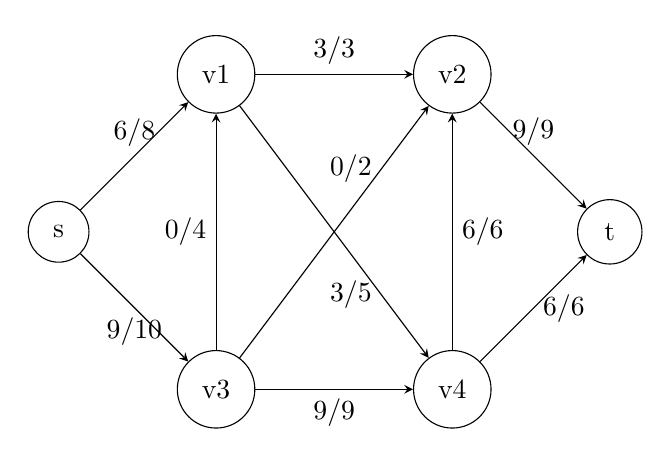
\begin{tikzpicture}[>=stealth]
        \node[ell] (s) at (0,0) {s};
        \node[ell] (v1) at (2,2) {v1};
        \node[ell] (v2) at (5,2) {v2};
        \node[ell] (v3) at (2,-2) {v3};
        \node[ell] (v4) at (5,-2) {v4};
        \node[ell] (t) at (7,0) {t};

        \draw [->] (s) to []node[above]{6/8} (v1);
        \draw [->] (s) to []node[below]{9/10} (v3);
        \draw [->] (v1) to []node[above]{3/3} (v2);
        \draw [->] (v1) to []node[left, near end]{3/5} (v4);
        \draw [->] (v2) to []node[above]{9/9} (t);
        \draw [->] (v3) to []node[left]{0/4} (v1);
        \draw [->] (v3) to []node[left, near end]{0/2} (v2);
        \draw [->] (v3) to []node[below]{9/9} (v4);
        \draw [->] (v4) to []node[right]{6/6} (v2);
        \draw [->] (v4) to []node[right]{6/6} (t);
    \end{tikzpicture}
    \end{subfigure}
\end{figure}
\end{problem}
\clearpage
\begin{problem}{3}
    A linear program is given as follows:\\\\
    Minimize $x_1+x_2+x_3$\\
subject to:\\
$2x_1 - 6x_2 + 3x_3 \geq 50$\\
$3x_1 + 4x_2 -x_3 \geq 40$\\
$4x_1 - x_2 + 5x_3 \geq 60$\\
$x_1, x_2 \geq 0$

\begin{enumerate}[label=(\alph*)]
    \item  Express the problem in either standard form or slack form\\
    standard form:\\
    Maximize $-x_1 - x_2 - x_3' + x_3''$\\
    $-2x_1 + 6x_2 - 3x_3' + 3x_3'' \leq -50$\\
    $-3x_1 - 4x_2 + x_3' - x_3'' \leq -40$\\
    $-4x_1 + x_2 - 5x_3' + 5x_3'' \leq -60$\\
    $x_1, x_2, x_3', x_3'' \geq 0$
    \item Solve the problem using a linear programming solver (e.g., linprog in python).
    \begin{lstlisting}[language=Python, caption=homework4.py]
# Import required libraries
import numpy as np
from scipy.optimize import linprog

# Set the inequality constraints matrix
# Note: the inequality constraints must be in the form of <=
A = np.array([[-2, 6, -3, 3], [-3, -4, 1, -1], [-4, 1, -5, 5],
    [-1, 0, 0, 0], [0, -1, 0, 0], [0, 0, -1, 0], [0, 0, 0, -1]])

# Set the inequality constraints vector
b = np.array([-50, -40, -60, 0, 0, 0, 0])

# Set the coefficients of the linear objective function vector
c = np.array([1, 1, 1, -1])

# Solve linear programming problem
res = linprog(c, A_ub=A, b_ub=b)

# Print results
print('Optimal value:', round(res.fun, ndigits=2),
'\nx values:', res.x,
'\nNumber of iterations performed:', res.nit,
'\nStatus:', res.message)
    \end{lstlisting}
    \begin{lstlisting}[language=C, caption=execution of homework4.py]
$python homework4.py
Optimal value: 21.82 
x values: [15.45454545  0.          6.36363636  0.        ] 
Number of iterations performed: 3
Status: Optimization terminated successfully. (HiGHS Status 7: Optimal)
    \end{lstlisting}
    \begin{enumerate}[label=(\alph*)]
        \item What is the optimum solution?\\
        $x_1+x_2+x_3=21.8181\ldots=\frac{240}{11}$
        \item What are the values of $x_1$, $x_2$, and $x_3$ for this optimum solution?\\
        $x_1 = 15.4545\ldots = \frac{170}{11},\;x_2=0,\;x_3=6.3636\ldots=\frac{70}{11}$
    \end{enumerate}
\end{enumerate}

\end{problem}


% --------------------------------------------------------------
%     You don't have to mess with anything below this line.
% --------------------------------------------------------------
 
\end{document}